\documentclass[border=4pt]{standalone}
\usepackage{tikz}
\begin{document}

\noindent
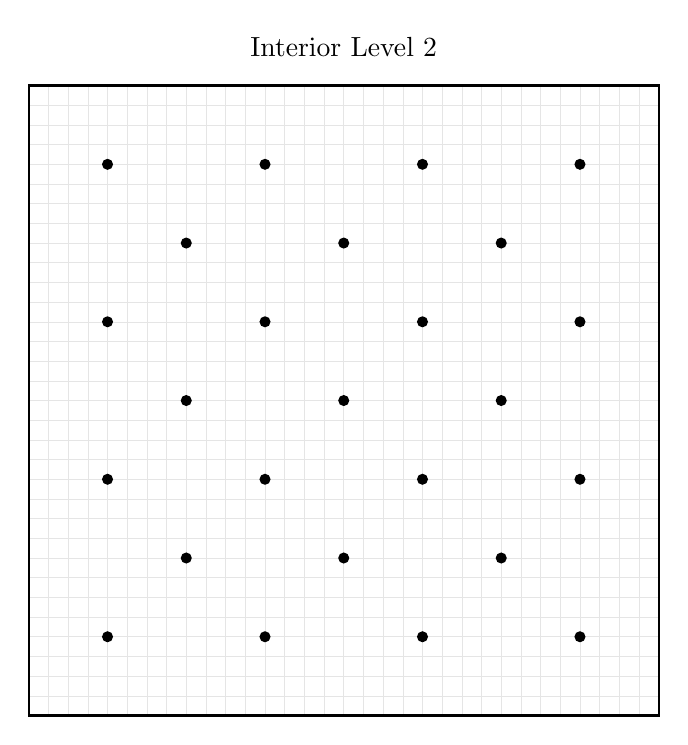
\begin{tikzpicture}[x=0.25cm,y=0.25cm]
  \draw[step=1,black!10,very thin] (0.0,0.0) grid (32.0,32.0);
  \draw[thick] (0,0) rectangle (32,32);
  \node (TOPL) at (16,33) [above,align=center]  {Interior Level 2};

%% (let* ((p 5)
%%        (m (expt 2 p))
%%        (s 8)
%%        (n (/ m s)))
%%   (cl-loop for x from 0 upto n
%%            do (cl-loop for y from 0 upto n
%%                        when (not (or (zerop x) (zerop y) (= n x) (= n y)))
%%                        do (insert (format "\\fill (%d,%d) circle(2pt);\n" (* s x) (* s y)))))
%%   (cl-loop for x from 0 upto (1- n)
%%            do (cl-loop for y from 0 upto (1- n)
%%                        do (insert (format "\\fill (%d,%d) circle(2pt);\n" (+ (/ s 2) (* s x)) (+ (/ s 2) (* s y)))))))

\fill (8,8) circle(2pt);
\fill (8,16) circle(2pt);
\fill (8,24) circle(2pt);
\fill (16,8) circle(2pt);
\fill (16,16) circle(2pt);
\fill (16,24) circle(2pt);
\fill (24,8) circle(2pt);
\fill (24,16) circle(2pt);
\fill (24,24) circle(2pt);
\fill (4,4) circle(2pt);
\fill (4,12) circle(2pt);
\fill (4,20) circle(2pt);
\fill (4,28) circle(2pt);
\fill (12,4) circle(2pt);
\fill (12,12) circle(2pt);
\fill (12,20) circle(2pt);
\fill (12,28) circle(2pt);
\fill (20,4) circle(2pt);
\fill (20,12) circle(2pt);
\fill (20,20) circle(2pt);
\fill (20,28) circle(2pt);
\fill (28,4) circle(2pt);
\fill (28,12) circle(2pt);
\fill (28,20) circle(2pt);
\fill (28,28) circle(2pt);

\end{tikzpicture}

\end{document}




